\documentclass{report}
\usepackage[margin=1in]{geometry}
\usepackage{setspace}
\usepackage{times}
\title{
	\textsc{ \small
		Washington State University \\
		School of Electrical Engineering and Computer Science \\
		EE 352, Electrical Engineering Laboratory
	} \\
	{\textsc{\small Lab \#5}} \\
	Diode characterization and applications
}

\author{
	Name: Kevin Evans \\
	Partner: Jacob Hnatiak
}
\date{Due Date: February 23, 2020}


% start sections at 1 with subsections to 1.1, 1.2...
\renewcommand{\thesection}{\arabic{section}}

%alias for vpp/rms
\newcommand{\pp}{_{pp}}
\newcommand{\rms}{_{rms}}
\newcommand{\Vpp}{\V\pp}
\newcommand{\Vrms}{\V\rms}

\usepackage{siunitx}
\usepackage{threeparttable}
\usepackage{booktabs}
\usepackage{multirow}
\usepackage{graphicx}
\usepackage{float}
\usepackage{amssymb,amsmath}
\usepackage{physics,cancel}

\usepackage{steinmetz} % \phase{}
\usepackage{mathtools} % for '\mathclap' macro
\usepackage{caption,subcaption} %multiline captions; subfigures


\begin{document}
\maketitle

\section*{Lab Overview}
% what was the lab about and the outcome?
In this lab, we explored the various characteristics of three different diodes: a general purpose switching diode, a rectifying diode, and Zener diodes. The forward and reverse bias modes were studied and used in several circuit applications. We obtained the diode I-V characteristics. Then, we estimated $I_s$ and the $n$ value for the general purpose diode. We used diodes in several applications, including a voltage regulator circuit, a voltage clipper/limiter, and a voltage doubler.

%%%%%%%%%%%%%%%%%%%%%%%%%%%%%%%%%%%%%%%%%%%%%%%%%%%%%%%%%%%%%
\section{Diode forward characteristics}

\subsection{Purpose}
% purpose of the experiment and its specs and/or design requirements
In this experiment, the forward bias characteristics were studied using the 1N4001 and 1N914 diodes. As a result of the experiment, the diode parameters $I_S$ and $n$ were calculated.

\subsection{Theoretical background}
% background and its theory of operation, circuit diagrams, the main equations, results from the prelab
The current within the forward bias region can be described as \begin{equation}
	I_D = I_s \left( e^{V_D / n V_T} - 1\right) \approx I_s e^{{V_D}/{nV_T}} \label{eq:exp1fwd}
\end{equation}
where $I_S$, $n$, and $V_T$ are relatively constant and are specific to the diode's type and manufacturing. From \eqref{eq:exp1fwd}, we can rearrange this for the difference of two voltages and approximate the diode's dynamic resistance,
\begin{equation}
	r_D = \frac{ n V_T }{I_D}
\end{equation}
In this experiment, we will be constructing a simple circuit, shown in Figure \ref{fig:exp1ckt} below. This circuit was simulated using OrCAD's PSPICE simulator using diode models for the 1N914 and 1N4001 models in the EVAL library. In the simulation, the voltage supply was swept from \num{0} to \SI{15}{\V} (dc) and the diode current was plotted against the voltage across each diode. This is shown in Figure \ref{fig:exp1sim}.

\begin{figure}[H]
	\centering
	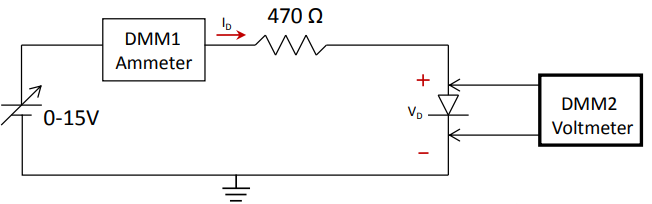
\includegraphics[width=0.7\linewidth]{exp1ckt}
	\caption{Circuit used for measuring the diode voltage and current.}
	\label{fig:exp1ckt}
\end{figure}

\begin{figure}[H]
	\centering
	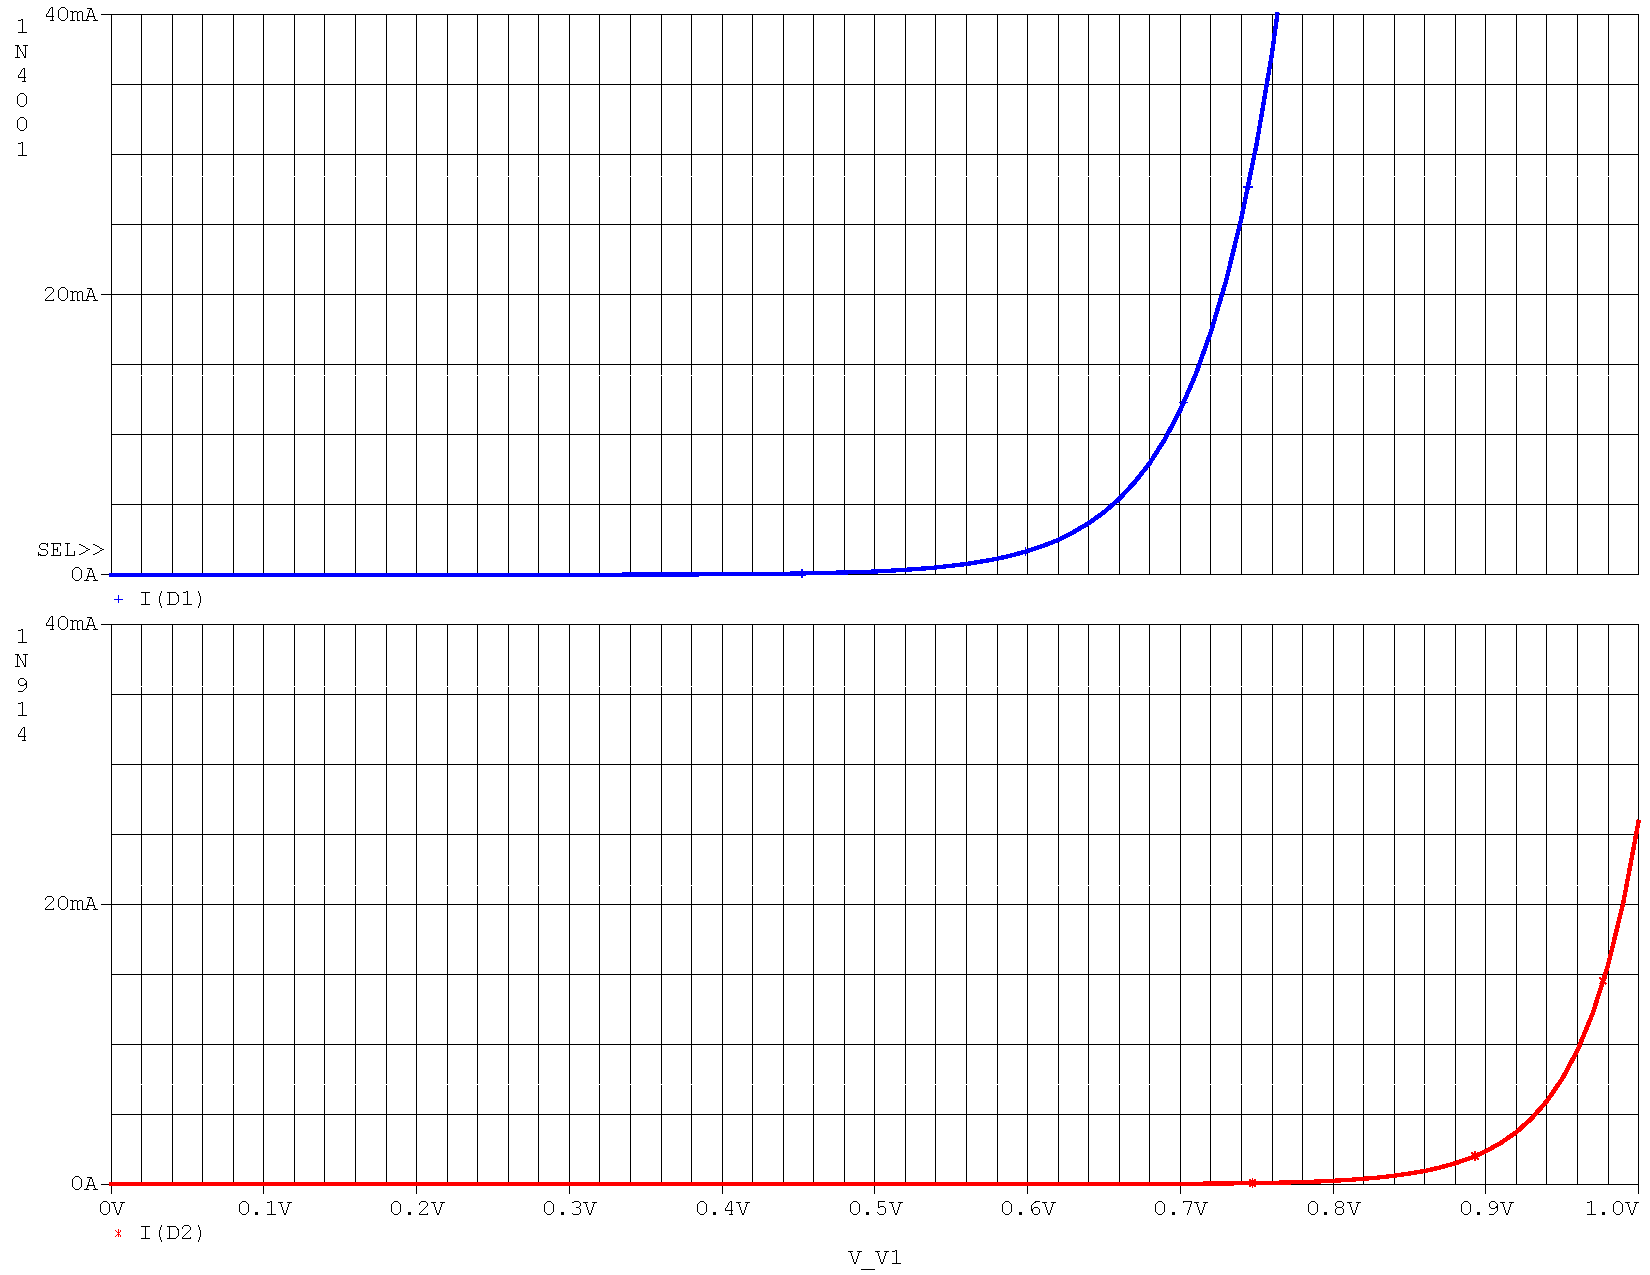
\includegraphics[width=1.0\linewidth]{exp1simcombined}
	\caption{Result of the simulation, plotting the diode current against the voltage across each diode. The models used in the simulation are the 1N4001 (top) and 1N914 (bottom) diode.}
	\label{fig:exp1sim}
\end{figure}

\subsection{Procedure}
The follow steps were carried out, as instructed by the lab assignment.
\begin{enumerate}
	\item The circuit shown in Figure \ref{fig:exp1ckt} was constructed and the resistor was measured.
	\item The dc voltage supply was used variably from \num{0} to \SI{15}{\V} and the voltage and current for the diode was recorded in Excel and plotted. This was then demonstrated to the TA.
	\item The TEK571 curve tracer was used for both diodes and pictures were taken.
	\item Using the diode equations and the data collected, the diode parameters $n$ and $I_s$ were estimated using \eqref{eq:exp1fwd} and data points near \SI{10}{\mA}.
	\item Using the $n$ and $I_s$ obtained, a PSPICE model was created for each diode and simulated. They were compared to the plots found in the previous steps.
	\item Using a least-squares fit, the data from Step 1 was fitted to an exponential model and the $n$ and $I_s$ values were calculated using the model.
\end{enumerate}

\subsection{Results and analysis}
% state all measured values, graphs, tables, and figs.
% state any deviation from theoretical expected values
% use tables and graphs
% * must justify error in results otherwise the experiment failed

\subsubsection{Circuit measurements}
The resistor $R$ was measured to be \SI{465.9}{\ohm} ($0.8\%$, within 5\% tolerance). Using a voltmeter across the diode and an ammeter in series, the data was collected for both diodes: 21 points for the 1N4001 diode and 16 points for the 1N914 diode. The points are plotted in Figure \ref{fig:exp1excel} below.
\begin{figure}[H]
	\centering
	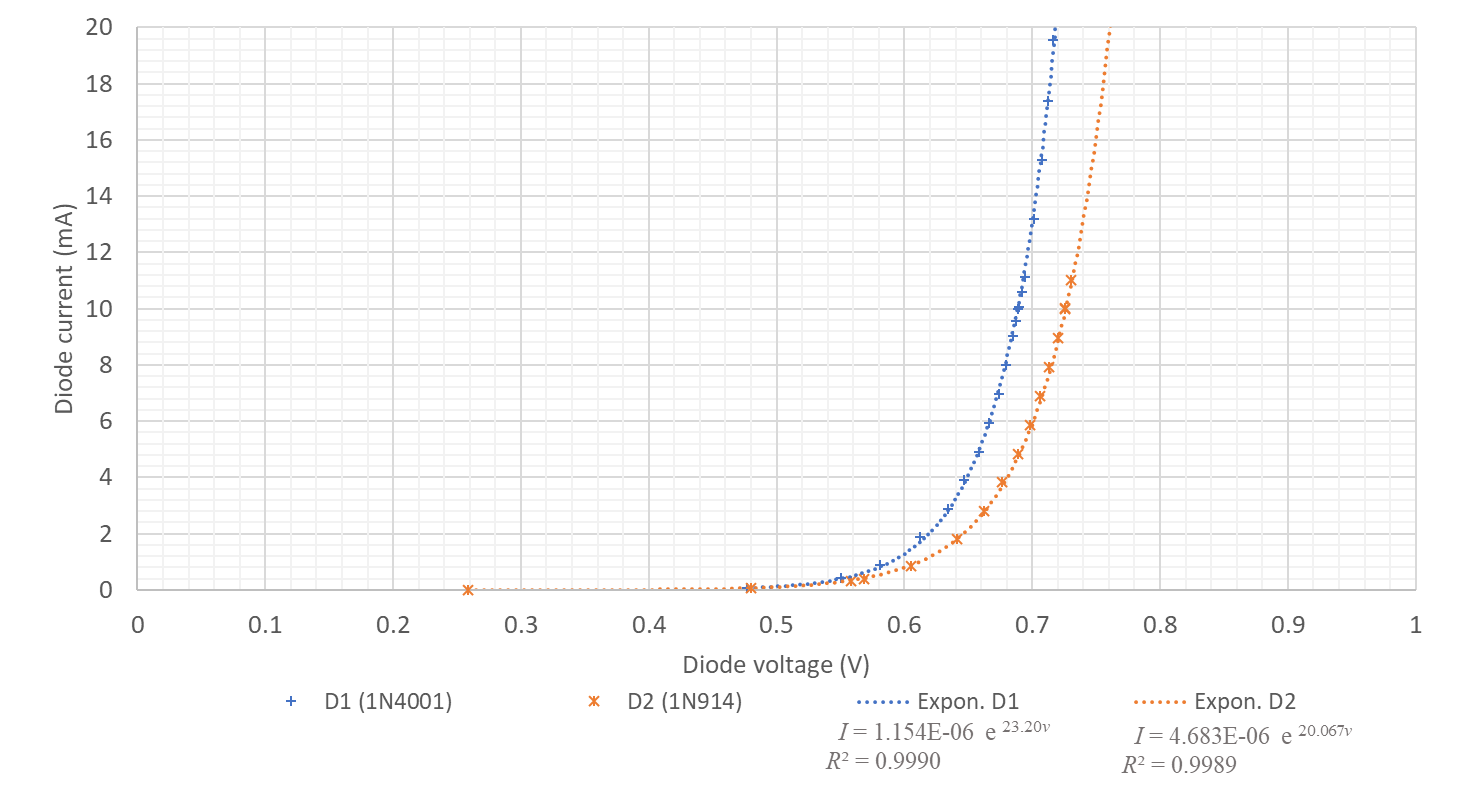
\includegraphics[width=1.0\linewidth]{exp1excel}
	\caption{The current-voltage characteristic curve of the 1N4001 and 1N914 diodes, and an exponential trendline.}
	\label{fig:exp1excel}
\end{figure}

Using measurements near \SI{10}{\mA}, the $n$ and $I_S$ values were calculated for both diodes. For each diode, we can use \eqref{eq:exp1fwd} and rearrange it for two points, \begin{align*}
	\Delta V & = n \left( \SI{26}{\mV} \right) \ln \frac{I_2}{I_1}
\end{align*}
The saturation current $I_S$ can be determined just from \eqref{eq:exp1fwd} and a single data point once $n$ is known. For the 1N4001, \begin{align*}
	n & = \frac{\SI{28}{\mV}}{\left(\SI{26}{\mV}\right) \ln 10.596/9.9999} \approx 1.857 \\
	I_S & = \SI{6.35}{\nA}
\end{align*}
Using the same method for the 1N914, \begin{align*}
	n & \approx 2.04 \\
	I_s & = \SI{11.5}{\nA}
\end{align*}

Using these $n$ and $I_S$ values, they were provided into the PSPICE model and the simulation was ran again, now with real-world values. The result of the simulation is closer than the original simulation but still has significant differences in the plots. The results are shown below in Figure \ref{fig:exp1postsim}.

The least-squares analysis provides a much more accurate result, rather than this analysis based on only two points. From the Tek 571 curve tracer, two pictures of the screens were taken. The Tek 571 produces a curve of the current-voltage relationship. The two diodes were tested and shown in Figure \ref{fig:exp1teks}, which provide a result nearly identical to the plots from Excel.

\begin{figure}[H]
	\centering
	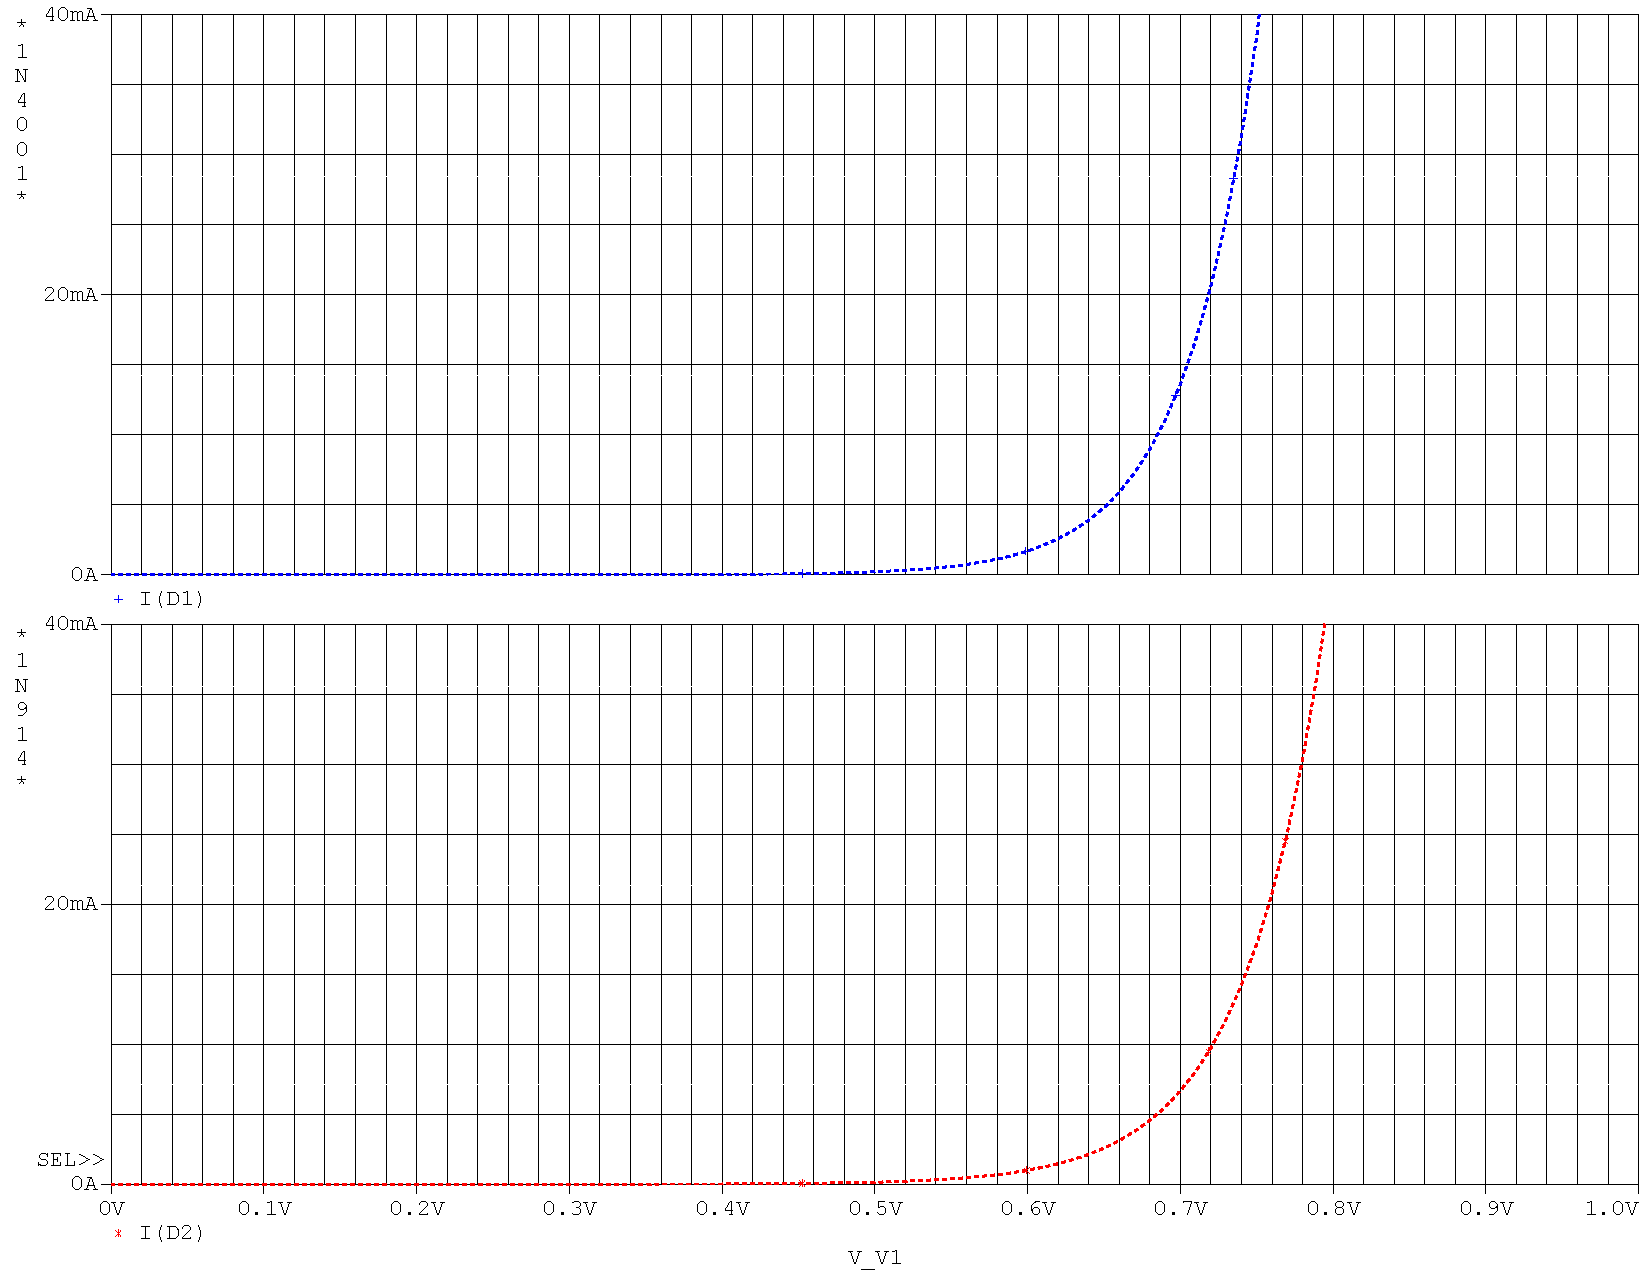
\includegraphics[width=1.0\linewidth]{exp1postsimcombined}
	\caption{Output of the simulation using the calculated $I_s$ and $n$ values.}
	\label{fig:exp1postsim}
\end{figure}

\begin{figure}[H]
	\begin{subfigure}{0.5\textwidth}
		\centering
		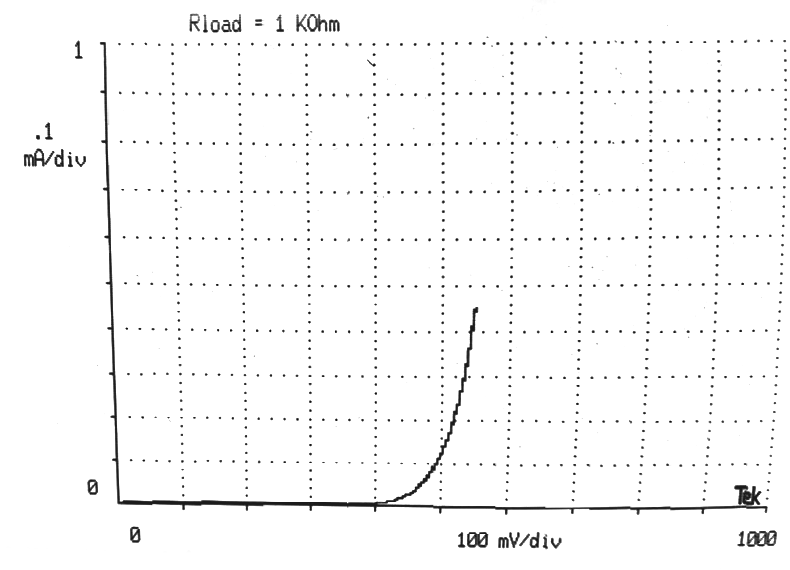
\includegraphics[width=\linewidth]{exp1tek1}
		\caption{}
		\label{fig:exp1tek1}
	\end{subfigure}
	\begin{subfigure}{0.5\textwidth}
		\centering
		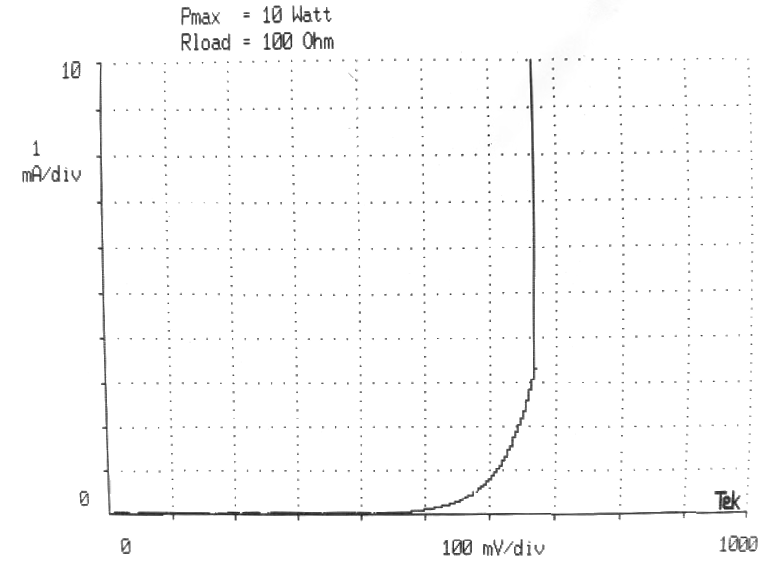
\includegraphics[width=\linewidth]{exp1tek2}
		\caption{}
		\label{fig:exp1tek2}
	\end{subfigure}
	\caption{Screenshots from the Tek 537, tracing the curves for the (a) 1N4001 and (b) 1N914. }
	\label{fig:exp1teks}
\end{figure}

\subsubsection{Least-squares exponential fit}
Within Excel, an exponential model was applied to the data, shown by the trendline in Figure \ref{fig:exp1excel}. From this, the saturation current and $n$-value can be determined. For the 1N4001, \begin{align*}
	I_D & = \left( \SI{1.154e-9}{\A}\right) e^{ \left( \SI{23.20}{\per\V}  \right) V_D} \\
		I_S & = \SI{1.154}{\nA} \\
		n & = \frac{1}{23.20 \times 0.026} = 1.66
\end{align*}
Similarly for the 1N914, \begin{align*}
	I_D & = \left( \SI{4.683e-9}{\A}\right) e^{ \left( \SI{20.607}{\per\V}  \right) V_D} \\
	I_S & = \SI{4.683e-9}{\nA} \\
	n & = 1.866
\end{align*}

\subsection{Conclusion}
%  conclusion of the exp
The forward bias characteristics of the 1N4001 and 1N914 diodes are modeled using the exponential \eqref{eq:exp1fwd}. The two parameters studied were the $n$ value and saturation current $I_S$. These characteristics describe how the diode responds in an I-V curve. The experimental result differed in some areas, but the minimal errors can be justified as the datasheet only describes the ideal diode. 

\pagebreak
%%%%%%%%%%%%%%%%%%%%%%%%%%%%%%%%%%%%%%%%%%%%%%%%%%%%%%%%%%%%%
\section{Zener Diode Characteristics}

\subsection{Purpose}
% purpose of the experiment and its specs and/or design requirements
In this experiment, we will explore the voltage-current relationships using a Zener diode. 
\subsection{Theoretical background}
% background and its theory of operation, circuit diagrams, the main equations, results from the prelab
The Zener diode behaves normally in the forward bias, however in reverse bias, the Zener diode has special characteristics that allow for different use-cases than the normal switching diode. IN reverse bias, the Zener diode allows a minuscule amount of current until it reaches the Zener-knee voltage $V_{zk}$. Past the knee voltage, there is a nearly linear relationship between voltage and current. From the 1N4735 datasheet, the ideal values were obtained for: \begin{align*}
	I_T & = \SI{41}{\mA} && \text{Test current} \\
	V_T & = \SI{6.2}{\V} && \text{Test voltage} \\
	r_z & = \SI{2.0}{\ohm} && \text{Dynamic resistance} \\
	I_{zk} & = \SI{1.0}{\mA} && \text{Min. knee current}\\
\end{align*}
Using the linear relationship in the Zener region, \begin{equation}
	V_Z = V_{z0} + I_Z r_z \label{eq:exp3vz}
\end{equation}
we can estimate the knee voltage as \begin{align}
	V_{ZK} \approx V_{Z0} & = V_Z - I_Z r_Z \notag \\
		& = 6.2 - (41 / 1000)(2.0) \notag \\
		& = \SI{6.118}{\V} \notag
\end{align}

\begin{figure}[H]
	\centering
	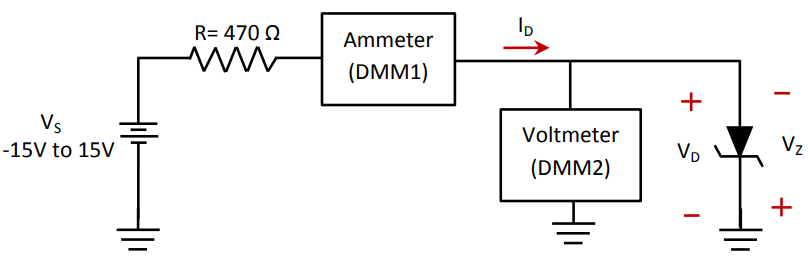
\includegraphics[width=0.7\linewidth]{exp2ckt}
	\caption{The circuit used to estimate the Zener characteristics in this experiment.}
	\label{fig:exp2ckt}
\end{figure}

\subsection{Procedure}
The follow steps were carried out, as instructed by the lab assignment.
\begin{enumerate}
	\item The circuit shown in Figure \ref{fig:exp2ckt} was constructed. Resistor $R$ was reused from the earlier experiment. The diode used was a Zener-type 1N4735. The voltage source $V_s$ was swept through $\pm \SI{15}{\V}$ (dc) and 34 points were collected.
	\item From the data collected, the minimum current $I_Z$ was estimated at the point where the plot enters the linear region.
	\item A value for $V_{Z0}$ and $r_Z$ were obtained by selecting two points in the linear region.
	\item The circuit was demonstrated to the TA.
\end{enumerate}

\subsection{Results and analysis}
% state all measured values, graphs, tables, and figs.
% state any deviation from theoretical expected values
% use tables and graphs
% * must justify error in results otherwise the experiment failed
The resistor from Experiment 1 was reused, with $R=\SI{465.9}{\ohm}$. The diode's current and voltage were collected at various points along the voltage sweep, with attention spent around the Zener region. This data was then plotted, shown in Figure \ref{fig:exp2plot} below. From the plot, the minimum Zener current $I_Z$ was estimated to be \SI{-0.99}{\mA} at \SI{6.032}{\V}
\begin{figure}[H]
	\centering
	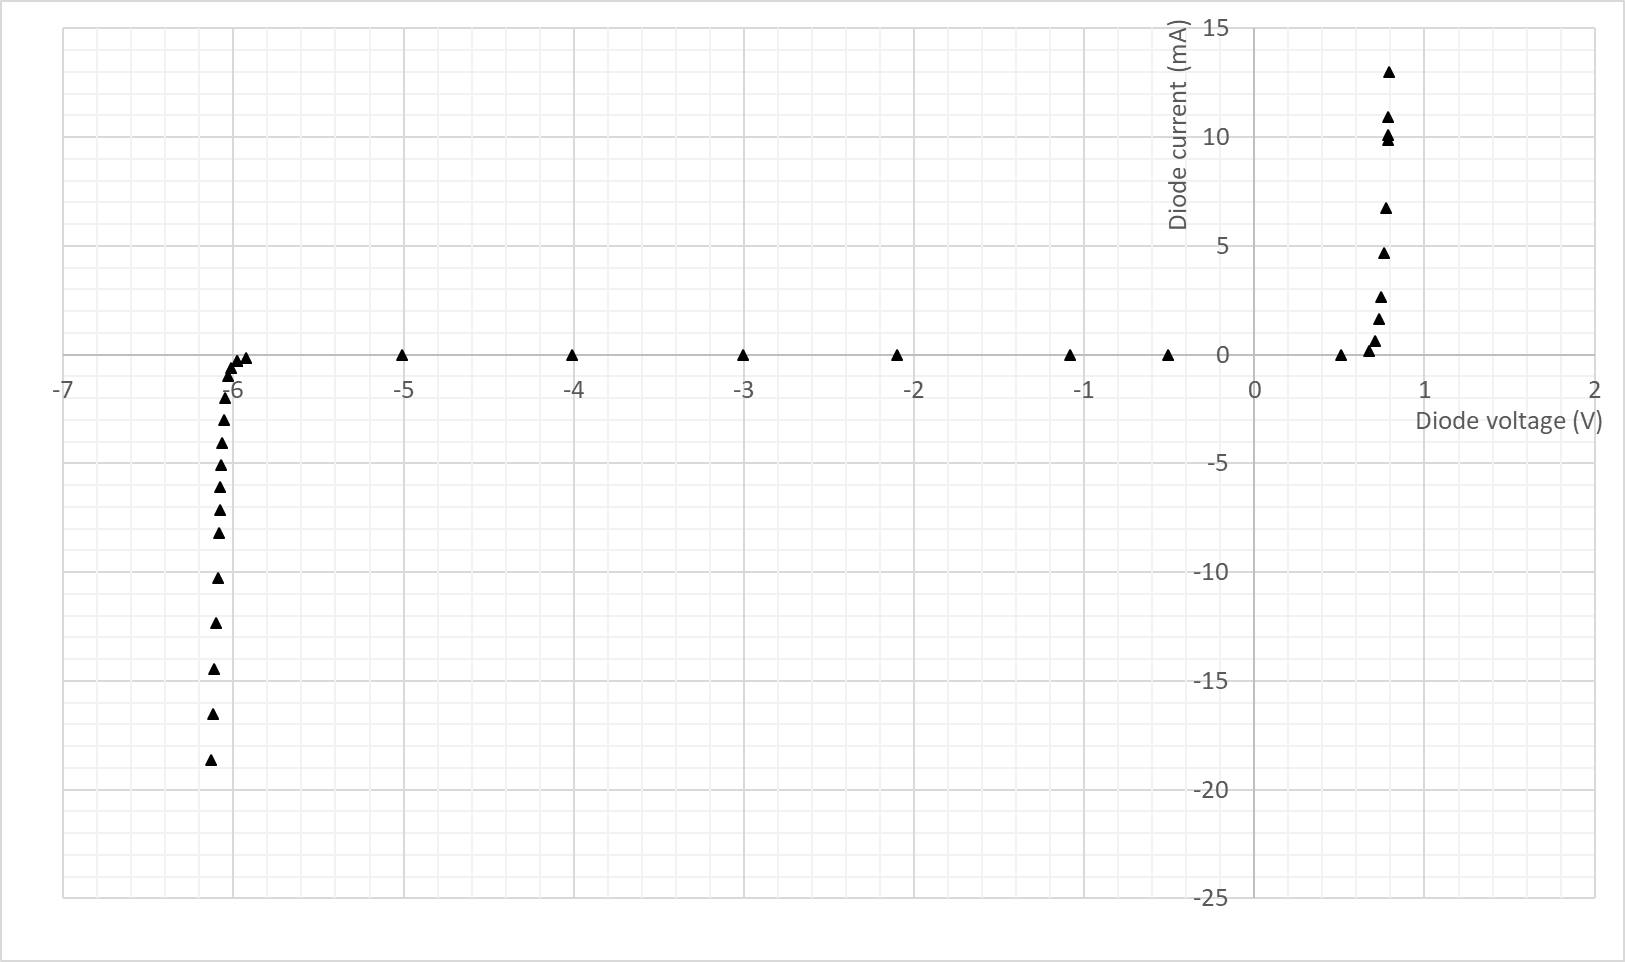
\includegraphics[width=\linewidth]{exp2plot}
	\caption{Plot of the Zener current and voltage of the 1N4735 diode.}
	\label{fig:exp2plot}
\end{figure}
\noindent Two points within the linear region were selected, \begin{align*}
	P_1 &(\SI{-6.071}{\V}, \SI{-5.085}{\mA}) \\
	P_2 & (\SI{-6.076}{\V}, \SI{-6.106}{\mA})
	\intertext{Modifying \eqref{eq:exp3vz}, the dynamic resistance of the Zener diode can be calculated as}
	r_Z & = \frac{\Delta V}{\Delta I} \\
		& = \frac{\SI{5}{\mV}}{\SI{1.021}{\mA}} \\
		& \approx \SI{4.9}{\ohm}
\end{align*}
The dynamic resistance $r_Z$ was substantially higher than the expected \SI{2}{\ohm}, exceeding 145\% error. The high error was likely due to the testing conditions for this dynamic resistance. In our test, the \SI{470}{\ohm} resistor limited the current to a maximum of \SI{30}{\mA}. However, at this current, the \SI{1/4}{\W} resistor would have melted.

From the datasheet, the Zener test current was \SI{41}{\mA}. It is likely that our experimental circuit limited the current and voltage enough so that it may not be in a truly linear region. To test this further would require choosing different voltage and resistor values to achieve a higher testing current.

\subsection{Conclusion}
%  conclusion of the exp
The Zener diode can easily be modeled using a linear fit, assuming the voltage is within the Zener region. The 1N4735 Zener diode in the experiment was found to have a higher experimental dynamic resistance, but this may be due to testing the diode below the test current used in the datasheet.
%%%%%%%%%%%%%%%%%%%%%%%%%%%%%%%%%%%%%%%%%%%%%%%%%%%%%%%%%%%%%
\section{Voltage Regulator}

\subsection{Purpose}
% purpose of the experiment and its specs and/or design requirements
The purpose of this experiment was to design a voltage regulator to supply a steady \SI{6.1}{\V} dc using the 1N4735 Zener diode, and values obtained from the previous experiment.

\subsection{Theoretical background}
% background and its theory of operation, circuit diagrams, the main equations, results from the prelab
Using the Zener shunt regulator circuit in Figure \ref{fig:exp3ckt}, a voltage regulator will be designed following the specifications: \begin{itemize}
	\item Input: \SI{9.5}{\V} DC $\pm \SI{0.5}{\V}$ @\SI{60}{\Hz}
	\item Output: \SI{6.1}{\V} DC, \SI{10}{\mA} (max)
	\item Zener diode: 1N4735, specifications: \begin{itemize}
			\item $V_Z = \SI{6.2}{\V}$
			\item $r_Z = \SI{2.0}{\ohm}$ at \SI{41}{\mA}
			\item $I_{ZK} = \SI{1}{\mA}$
			\item $V_{Z0} = \SI{6.118}{\V}$
		\end{itemize}
\end{itemize}
To begin designing this regulator, we will look at the worst-case where: \begin{itemize}
	\item The load current is maximum (\SI{10}{\mA})	
	\item The Zener current is maintained at $\ge \SI{5}{\mA}$
	\item The supply voltage is at its lowest (\SI{9.0}{\V}), where the current supplied will therefore be at its lowest point
\end{itemize}
The current through the resistor will be \begin{align*}
	I_R & = 5 + 10 = \SI{15}{\mA}
	\intertext{We can use Ohm's law and the Zener I-V relationship,}
	I_R & = \frac{V_s - V_z}{R} \\
		& = \frac{V_s - (V_{Z0} + I_z r_Z)}{R} && \text{Using \eqref{eq:exp3vz}}
	\intertext{Using the values from earlier, we can then solve for the resistance $R$,}
	\SI{15}{\mA} & = \frac{9.0 - \left(6.118 + (5 / 1000) 2 \right)}{R} \\
	R & = \SI{191.5}{\ohm}
\end{align*}
\begin{figure}[H]
	\centering
	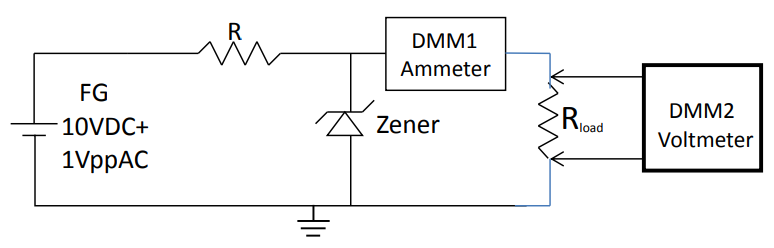
\includegraphics[width=0.7\linewidth]{exp3ckt}
	\caption{The Zener-shunt voltage regulator circuit used in Experiment 3.}
	\label{fig:exp3ckt}
\end{figure}
\subsection{Procedure}
The follow steps were carried out, as instructed by the lab assignment.
\begin{enumerate}
	\item The circuit shown in Figure \ref{fig:exp3ckt} was constructed with $R=\SI{191.5}{\ohm}$ (nominal). The effect of a load current on the load voltage was investigated with an input power supply of \SI{9.5}{\V} dc. This was accomplished using the function generator set to \SI{9.5}{\V} dc offset with \SI{2}{\mV} (pp) AC at \SI{60}{\Hz}.
	
	\item Using the decade box as the variable resistor, this was attached as the load resistor. The dc load voltage and current was measured from \num{0} to \SI{10}{\mA} in 10 steps. This was accomplished by varying the decade box resistance until these currents were reached. Each data point was recorded in Excel and plotted.
	\item The circuit and the plots were verified and demonstrated to the TA.
	\item Next, the effect of AC ripple was investigated. The load current was set to \SI{5}{\mA} and the AC wave was set to \SI{1}{\Vpp}. With the scope, the ripple voltage was measured and the ratio of output to input ripple was calculated.
\end{enumerate}

\subsection{Results and analysis}
% state all measured values, graphs, tables, and figs.
% state any deviation from theoretical expected values
% use tables and graphs
% * must justify error in results otherwise the experiment failed
As \SI{191.5}{\ohm} nominal resistors were unavailable, we chose two \SI{100}{\ohm} 5\% resistors in series. The two resistors had a measured equivalent resistance of $R=\SI{197.0}{\ohm}$, 2.6\% error from the target. We plotted the specified range of Zener voltages and currents, resulting in the plot in Figure \ref{fig:exp3plot}.
\begin{figure}[h]
	\centering
	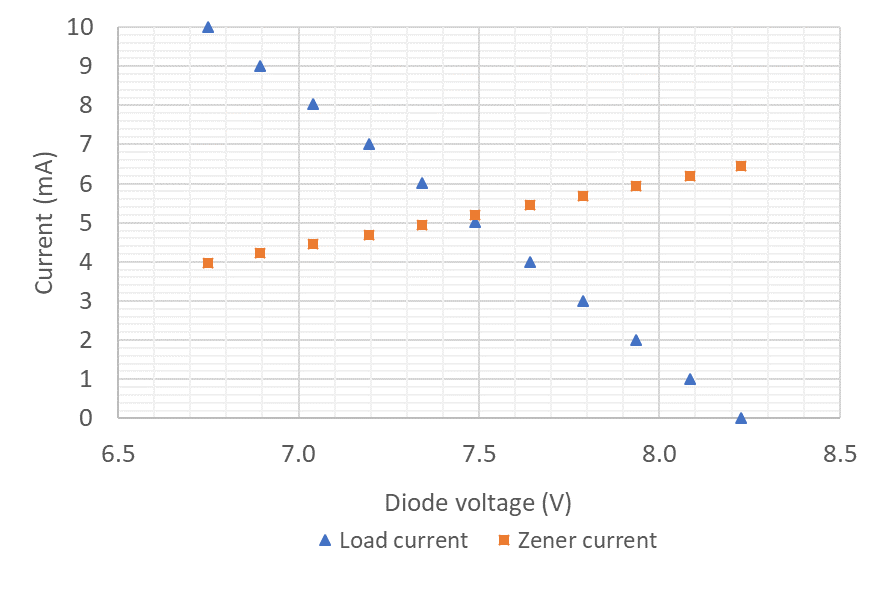
\includegraphics[width=0.7\linewidth]{exp3plot}
	\caption{Plot of the load and Zener currents, both versus the diode voltage.}
	\label{fig:exp3plot}
\end{figure}

After adjusting the input to include the AC \SI{1}{\Vpp} ripple, we observed a ripple shown in Figure \ref{fig:exp3ripple}. The ripple voltage was measured using the 1X probe as \SI{640}{\uV} (pp). The output ripple is quite small and shows a fairly effective attempt at line regulation. The ratio of output ripple is calculated as
\[ \frac{V_{Rout}}{V_{Rin}} = \frac{\SI{640}{\uV}}{\SI{1}{\V}} = \SI{640e-6}{\V/\V} \]

\begin{figure}[h]
	\centering
	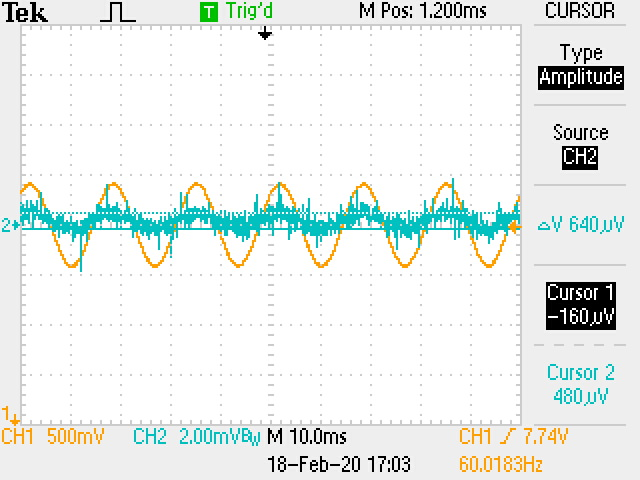
\includegraphics[width=0.4\linewidth]{exp3ripple}
	\caption{The output ripple voltage of the regulator.}
	\label{fig:exp3ripple}
\end{figure}

\subsection{Conclusion}
%  conclusion of the exp
This experiment showed another application of a Zener diode: the Zener shunt regulator. This regulator was found to have a fairly effective line regulation, with a \num{640e-6} output to input ratio of ripple. 

\pagebreak
%%%%%%%%%%%%%%%%%%%%%%%%%%%%%%%%%%%%%%%%%%%%%%%%%%%%%%%%%%%%%
\section{Voltage limiting/clipping circuit}

\subsection{Purpose}
% purpose of the experiment and its specs and/or design requirements
The purpose of this experiment was to build a circuit to limit a voltage using diodes. In this application of the forward-bias diode, once a voltage exceeds a threshold, it is fed back across a resistor.

\subsection{Theoretical background}
% background and its theory of operation, circuit diagrams, the main equations, results from the prelab
In this experiment, we will be applying sine waves at $\SI{1}{\kHz}$ and assuming a \SI{0.7}{\V} drop across diodes. The circuit used in this experiment is shown in Figure \ref{fig:exp4ckt} below. 
\begin{figure}[H]
	\centering
	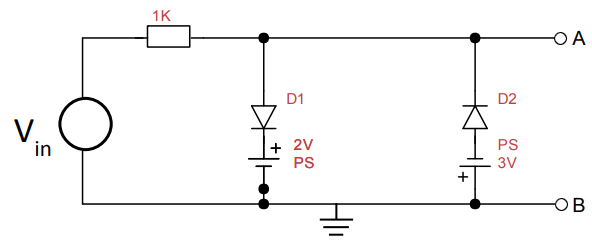
\includegraphics[width=0.6\linewidth]{exp4ckt}
	\caption{The circuit used to demonstrate voltage clipping in Experiment 4.}
	\label{fig:exp4ckt}
\end{figure}
The output voltage $V_{AB}$ can be described using a piecewise as, \begin{equation}
	V_{AB} = \begin{cases}
		V_{in} & -3.7 < V_{in} < 2.7 \\
		2.7 & V_{in} > 2.7 \\
		-3.7 & V_{in} < -3.7
	\end{cases}
\end{equation}
Once the voltage exceeds these limits, it is exceeding the threshold of the forward bias and the diodes allow current to flow across $R$, assuming $AB$ is an open circuit or has a high resistance. If we take the input sine waveforms at $\SI{1}{\kHz}$ with peak-peak magnitudes of \num{2}, \num{7}, and \SI{10}{\V}, we can estimate the output $AB$, assuming ideal waves as shown in Figure \ref{fig:exp4waveforms}.
\begin{figure}[h]
	\centering
	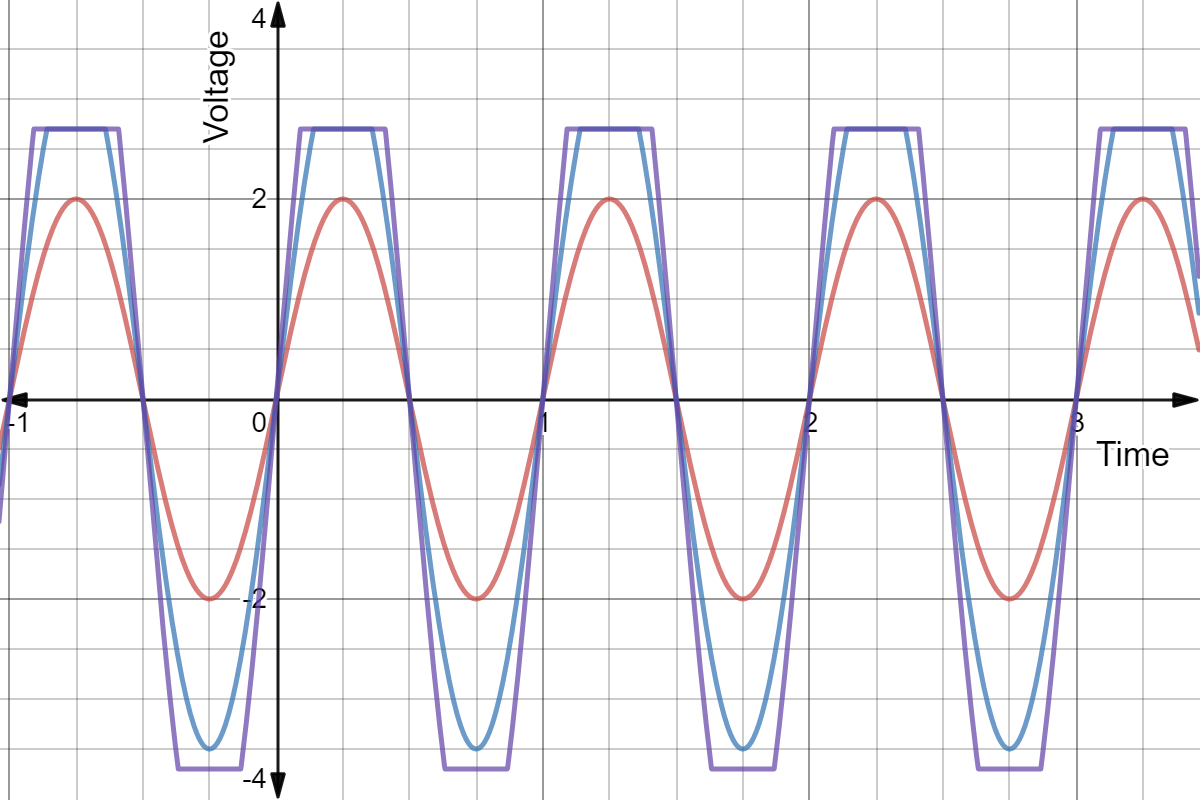
\includegraphics[width=0.4\linewidth]{exp4waveforms}
	\caption{The expected clipping, if the voltage drop is assumed constant.}
	\label{fig:exp4waveforms}
\end{figure}
\subsection{Procedure}
The follow steps were carried out, as instructed by the lab assignment.
\begin{enumerate}
	\item The circuit shown in Figure \ref{fig:exp4ckt} was constructed using two 1N914 diodes. The resistor was measured. Two dc power supplies were attached, the first at \SI{2}{\V} and the other at \SI{3}{\V}.
	\item The function generator was initialized for a \SI{1}{\kHz} sine wave at \SI{2}{\Vpp}, \SI{7}{\Vpp}, and \SI{10}{\Vpp}. Clipping was observed and screenshots were taken.
	\item The output waveforms were compared to the expected waveforms.
\end{enumerate}

\subsection{Results and analysis}
% state all measured values, graphs, tables, and figs.
% state any deviation from theoretical expected values
% use tables and graphs
% * must justify error in results otherwise the experiment failed
The resistor was measured to be $R=\SI{973.6}{\ohm}$ (2.6\% error). As expected, clipping was observed on the \SI{7}{\Vpp} and \SI{10}{\Vpp} input waves. However, the clipping level was different than the prelab expectations.

At \SI{7}{\Vpp}, the positive half of the wave clipped at \SI{2.76}{\V}, 2\% from the expected value. From the \SI{10}{\Vpp} wave, the positive half clipped at \SI{3}{\V} and the negative half clipped at \SI{-3.24}{\V}, exceeding the expected value by 11\% and 12\% respectively. 

The deviation is likely due to the limitations of the constant-drop model and the fact that the diodes affect each other. The diodes simply use the voltage differences between the cathode and anode; when one diode allows current to flow across, it affects the second diode and vice-versa.

\begin{figure}[h]
	\centering
	\begin{subfigure}{0.3\textwidth}
		\centering
		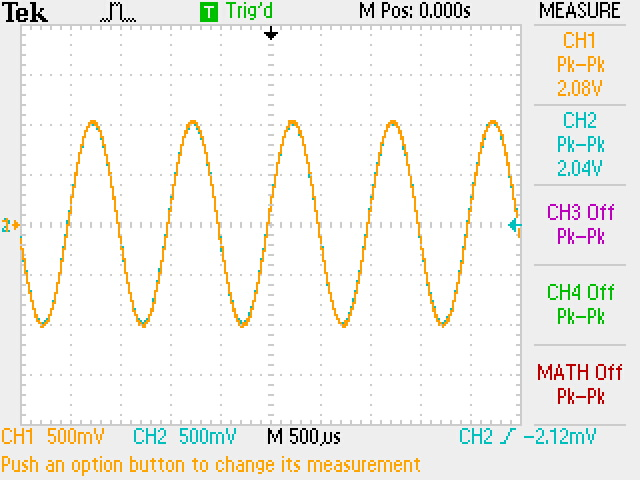
\includegraphics[width=\linewidth]{exp4_a}
		\caption{\SI{2}{\Vpp}}
		\label{fig:exp4a}
	\end{subfigure}
	\begin{subfigure}{0.3\textwidth}
		\centering
		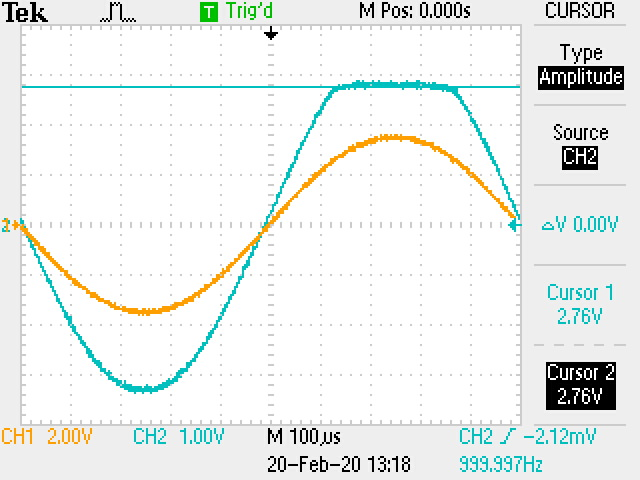
\includegraphics[width=\linewidth]{exp4_b}
		\caption{\SI{7}{\Vpp}}
		\label{fig:exp4b}
	\end{subfigure}
	\begin{subfigure}{0.3\textwidth}
		\centering
		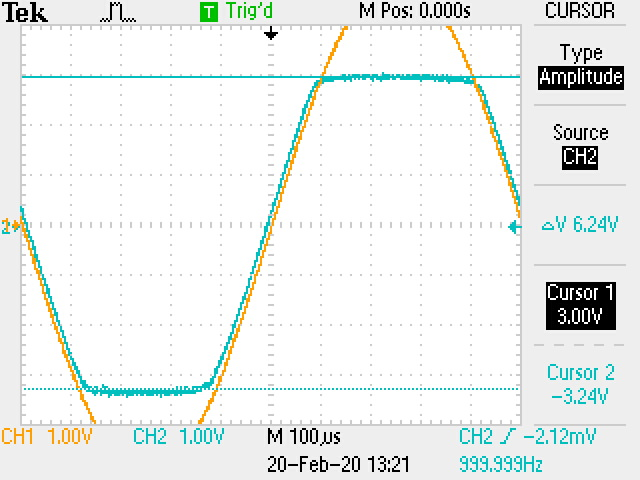
\includegraphics[width=\linewidth]{exp4_c}
		\caption{\SI{10}{\Vpp}}
		\label{fig:exp4c}
	\end{subfigure}

	\caption{Output waveforms measured on the oscilloscope.}
\end{figure}
\subsection{Conclusion}
This experiment demonstrated another use of diodes: voltage clipping. The diode can be used to limit the maximum and minimum voltage on a node in a circuit. In this case, we set the approximate maximum and minimum voltage for an AC input. However, there are some caveats as a constant voltage drop model cannot always be used. Assuming a constant drop of 0.7V led to errors, visible in the oscilloscope screenshots above. More consideration is needed when multiple diodes are expected to be forward biased.
%  conclusion of the exp

%%%%%%%%%%%%%%%%%%%%%%%%%%%%%%%%%%%%%%%%%%%%%%%%%%%%%%%%%%%%%
\section{Voltage Doubler}

\subsection{Purpose}
% purpose of the experiment and its specs and/or design requirements
This experiment demonstrates the voltage doubler circuit, allowing an input voltage to be essentially doubled using a network of capacitors and diodes. The ripple voltage is studied as well and the effect of larger capacitors is noted.

\subsection{Theoretical background}
% background and its theory of operation, circuit diagrams, the main equations, results from the prelab
The voltage doubler is a circuit used to nearly double an input voltage. This is accomplished by using an AC input and diodes as an effective check valve. Once current flows through a diode, the rectified voltage is seen by the capacitor and charge begins to accumulate during that half-cycle. The circuit in Figure \ref{fig:exp5ckt} demonstrates the voltage doubler and will be used in this experiment.
\begin{figure}[h]
	\centering
	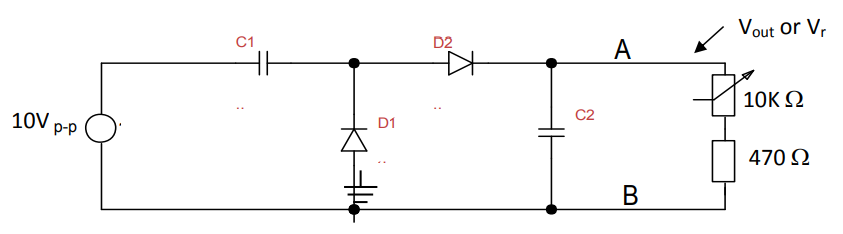
\includegraphics[width=0.7\linewidth]{exp5ckt}
	\caption{The voltage doubler circuit used in Experiment 5.}
	\label{fig:exp5ckt}
\end{figure}

In OrCAD PSPICE, we can simulate this voltage doubler circuit. This was done with no load (OC) and a resistive load of \SI{1}{\kohm} and capacitances of \SI{1}{\micro\farad}. At no load, the voltage steadily reaches equilibrium roughly around \SI{8.5}{\V}. With the load of \SI{1}{\kohm}, there is a massive swing in voltage as the capacitors are unable to keep up with the low resistive load. This causes a massive ripple due to current flowing out of the second capacitor and dissipating within the resistors. The average DC voltage is roughly around \SI{5}{\V}.

\begin{figure}[h]
	\begin{subfigure}{0.5\textwidth}
		\centering
		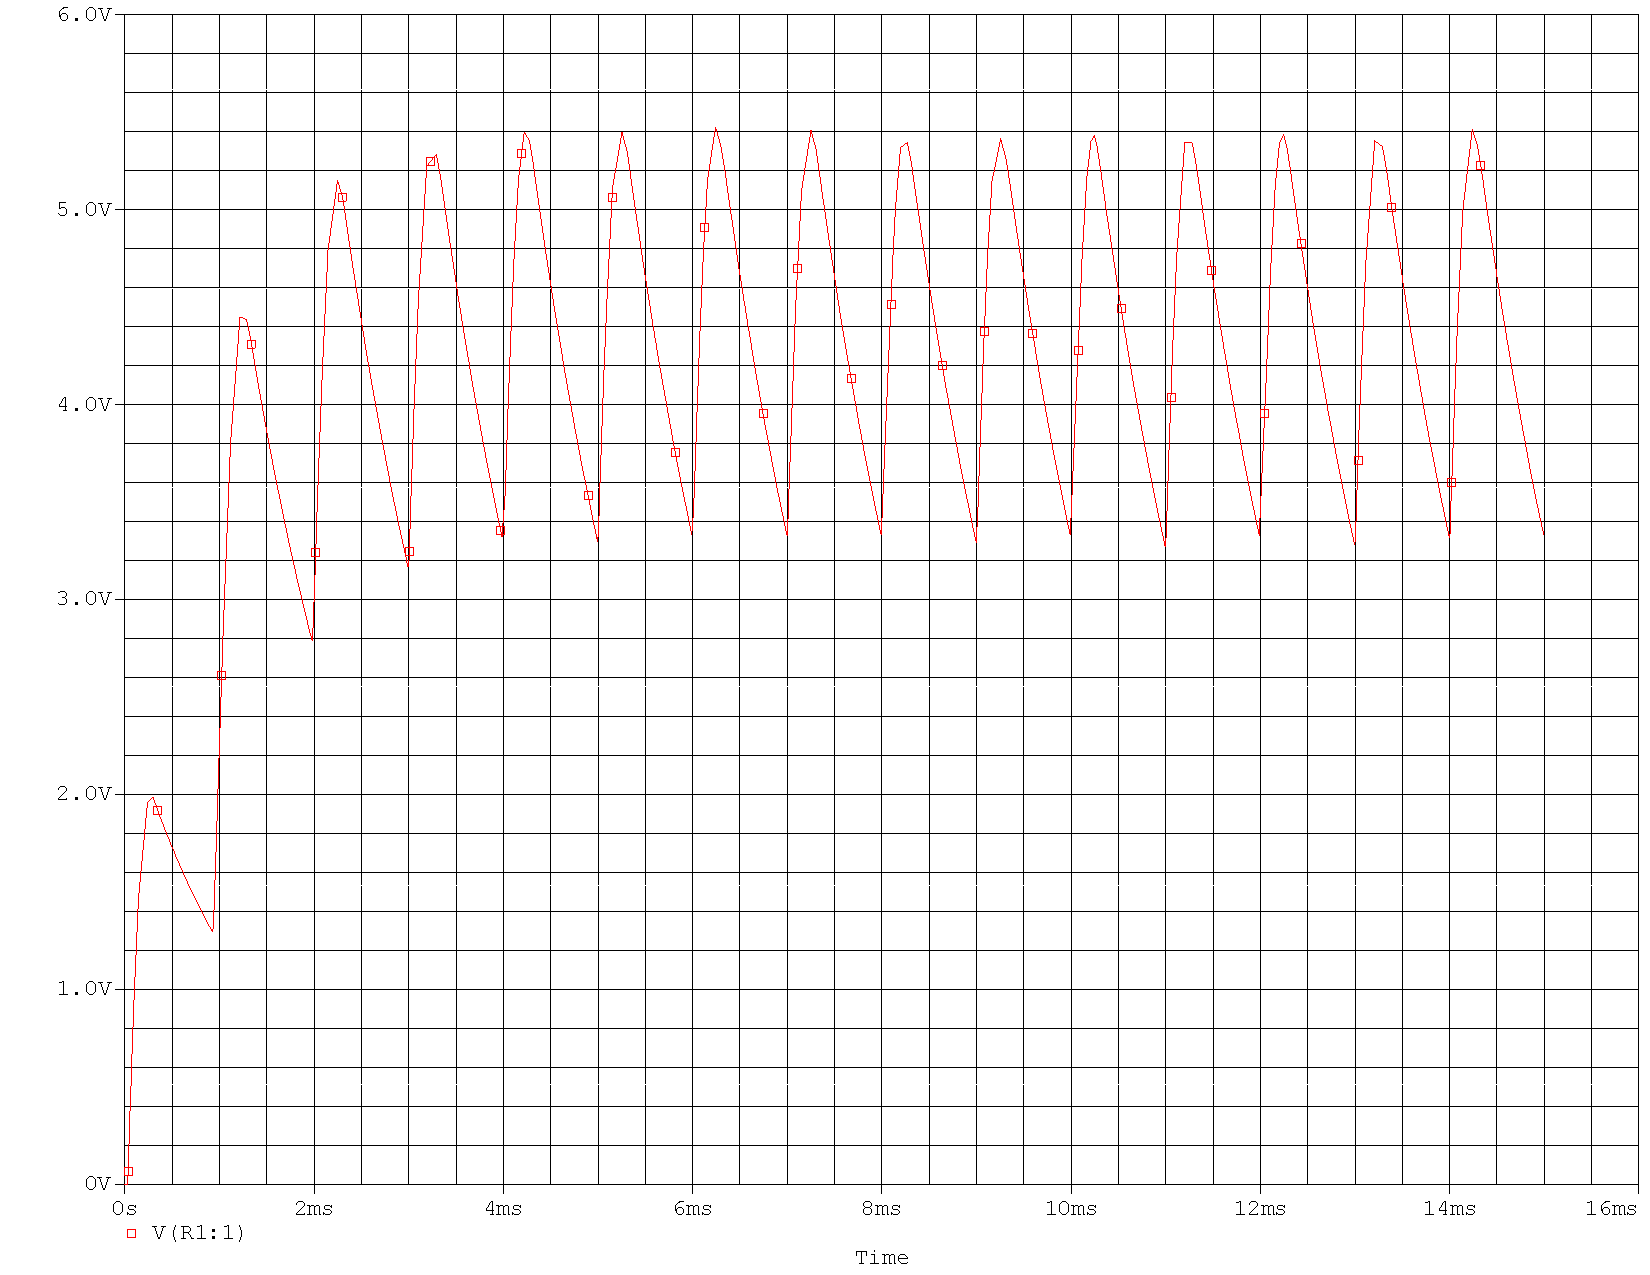
\includegraphics[width=\linewidth]{exp5load}
		\caption{}
		\label{fig:exp5load}
	\end{subfigure}
	\begin{subfigure}{0.5\textwidth}
		\centering
		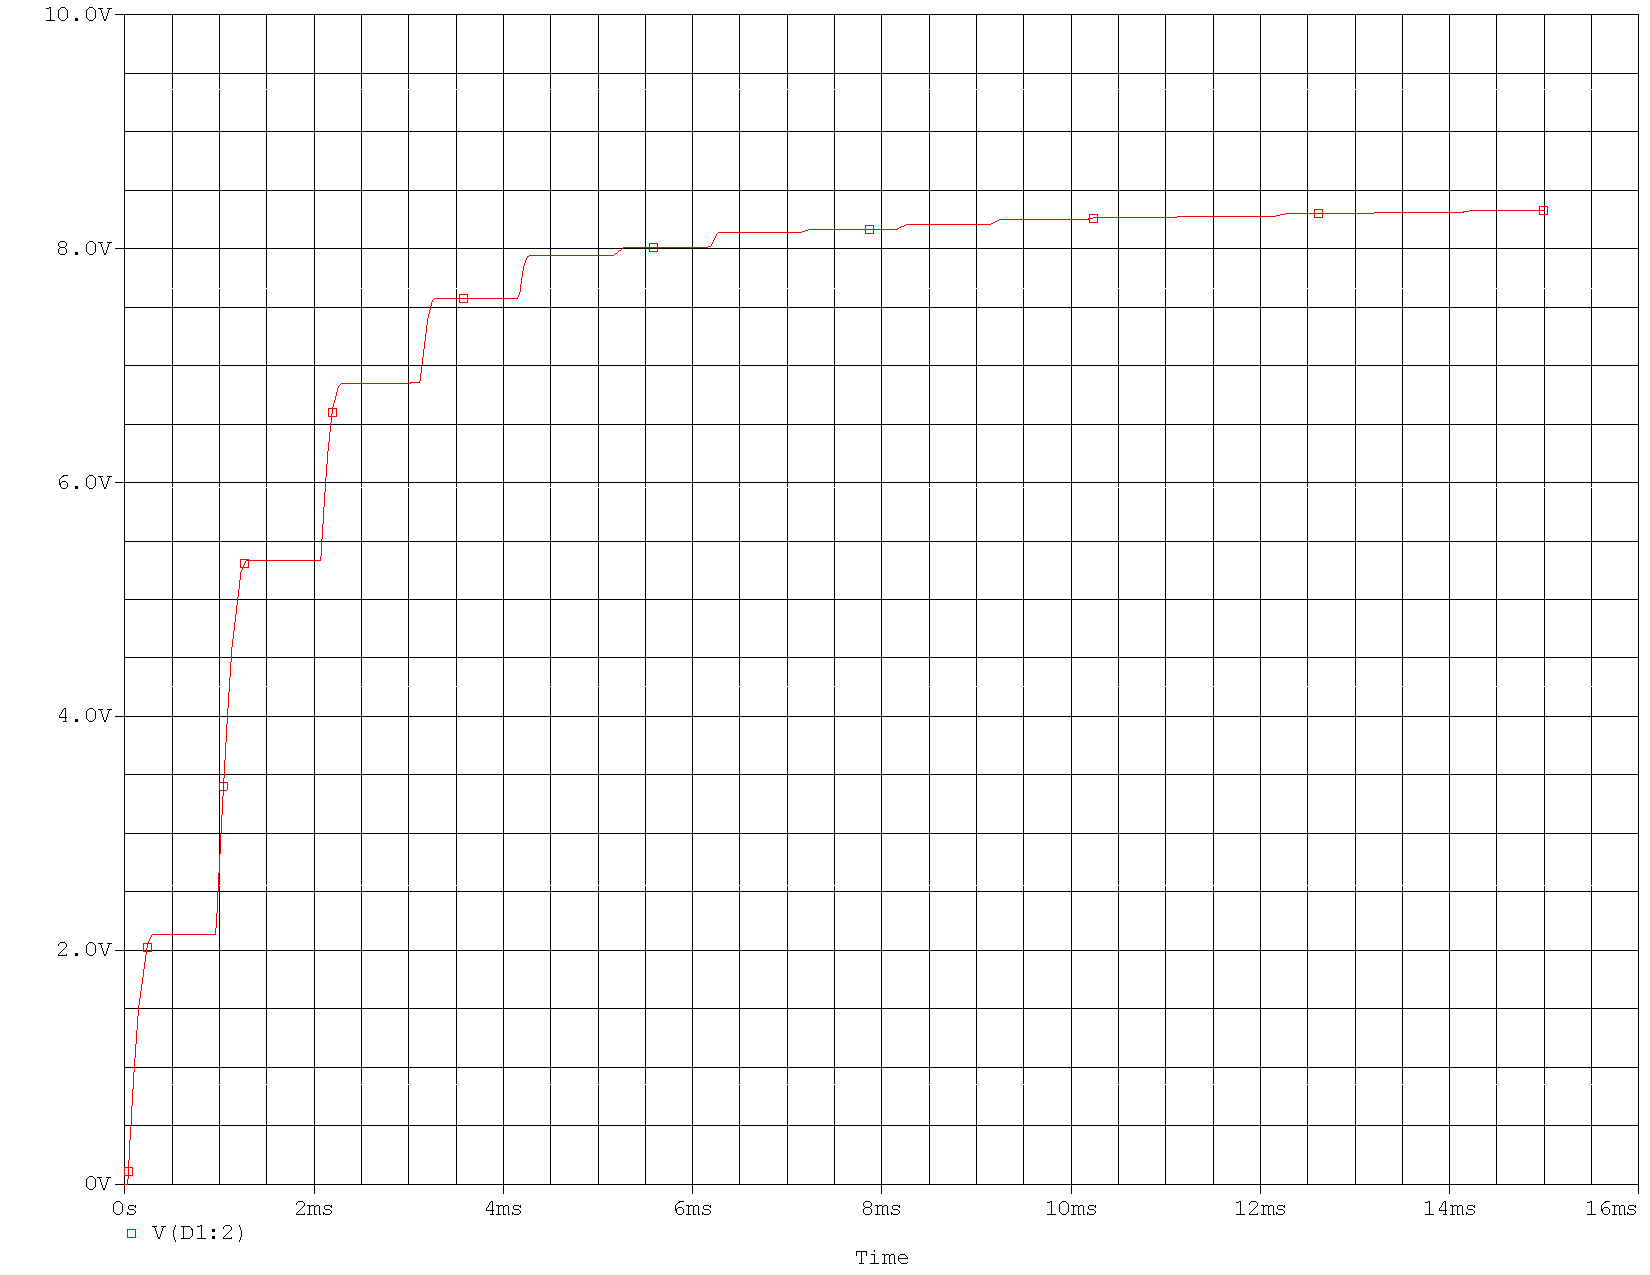
\includegraphics[width=\linewidth]{exp5noload}
		\caption{}
		\label{fig:exp5noload}
	\end{subfigure}
	\caption{Output voltage with (a) \SI{1}{\kohm} load resistor and (b) no load.}
	\label{fig:exp5sim}
\end{figure}
\pagebreak
\subsection{Procedure}
The follow steps were carried out, as instructed by the lab assignment.
\begin{enumerate}
	\item The circuit in Figure \ref{fig:exp5ckt} was constructed. The function generator was used an input with \SI{10}{\Vpp} sine wave at \SI{1}{\kHz}. The diode was chosen to be an 1N914 diode. The capacitors used were \SI{1}{\micro\farad} (nominal) electrolytic capacitors. The components were measured. The output voltage was measured with no load using the DMM.
	\item A \SI{470}{\ohm} and \SI{10}{\kohm} variable resistor was added as the load. The DMM was used to measure the output voltage $V_{out}$ and the oscilloscope with AC coupling was used measure the ripple voltage $V_r$. Ten readings were measured every $\SI{1}{\kohm}$ from \SI{470}{\ohm} upward.
	\item These steps were repeated for \SI{10}{\micro\farad} capacitors.
	\item The data was collected in Excel and plotted, with the ripple voltage and load voltages as functions of the resistance.
\end{enumerate}

\subsection{Results and analysis}
% state all measured values, graphs, tables, and figs.
% state any deviation from theoretical expected values
% use tables and graphs
% * must justify error in results otherwise the experiment failed

\subsubsection{Measured component values}
The components were measured and listed in Table \ref{table:lab5components} below.
\begin{table}[h]
	\centering
	\caption{Experimental and nominal component values.}
	\label{table:lab5components}
	\begin{threeparttable}
		\begin{tabular}{cccc}
			\toprule
			Component & Nominal & Experimental & \% Error (Tolerance) \\
			\midrule
			$R$ & \SI{470}{\ohm} & \SI{465.0}{\ohm} & 1.1\% (5\%)\\
			\midrule
			$C_1$  & \SI{1}{\micro\farad} & \SI{0.9126}{\micro\farad} & 4.1\%  \\
			$C_2$  & \SI{1}{\micro\farad} & \SI{0.9209}{\micro\farad} & 7.9\%  \\
			\midrule
			$C_1$  & \SI{10}{\micro\farad} & \SI{9.74}{\micro\farad} & 2.6\%  \\
			$C_2$  & \SI{10}{\micro\farad} & \SI{9.50}{\micro\farad} & 5.0\%  \\
			\bottomrule
		\end{tabular}
	\end{threeparttable}
\end{table}
\subsubsection{Circuit output voltage} 
With no load, the voltage was measured using the oscilloscope as
\[V_0 = \SI{9.21}{\V} \]
With the load $R$ and the resistor box, ten data points were plotted using Excel for both sets of capacitors, shown in Figure \ref{fig:exp5plotripple} and Figure \ref{fig:exp5plotdc}. At higher resistances, the ripple decreases and the DC voltage increases. This is entirely expected as it limits the current that can flow out of the capacitors; this is seen when looking at the time constant. As the resistance increases, the time constant increases, indicating the capacitor will discharge slower than a low resistance.
Similarly, as the capacitance increased from 1 to 10 microfarad, the capacitor is able to store more charge and retain a voltage longer. This is also seen in the time constant, which is proportional to the capacitance.

\begin{figure}[h]
	\centering
	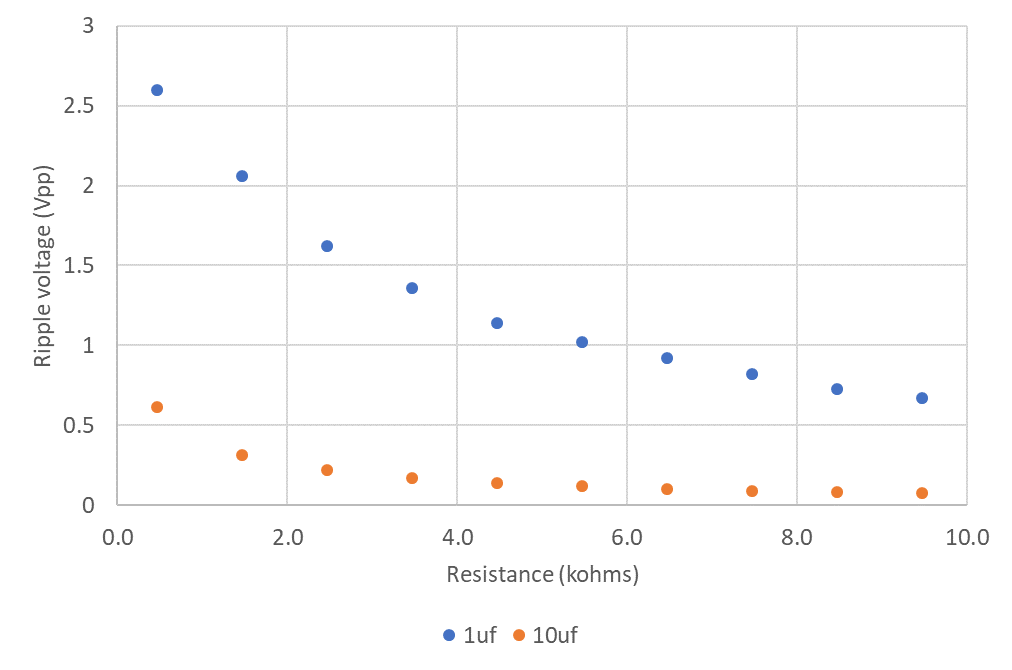
\includegraphics[width=0.7\linewidth]{exp5plotripple}
	\caption{The ripple versus the resistance. The higher the resistance, the less current flows, and the lower the ripple becomes.}
	\label{fig:exp5plotripple}
\end{figure}
\begin{figure}[h]
	\centering
	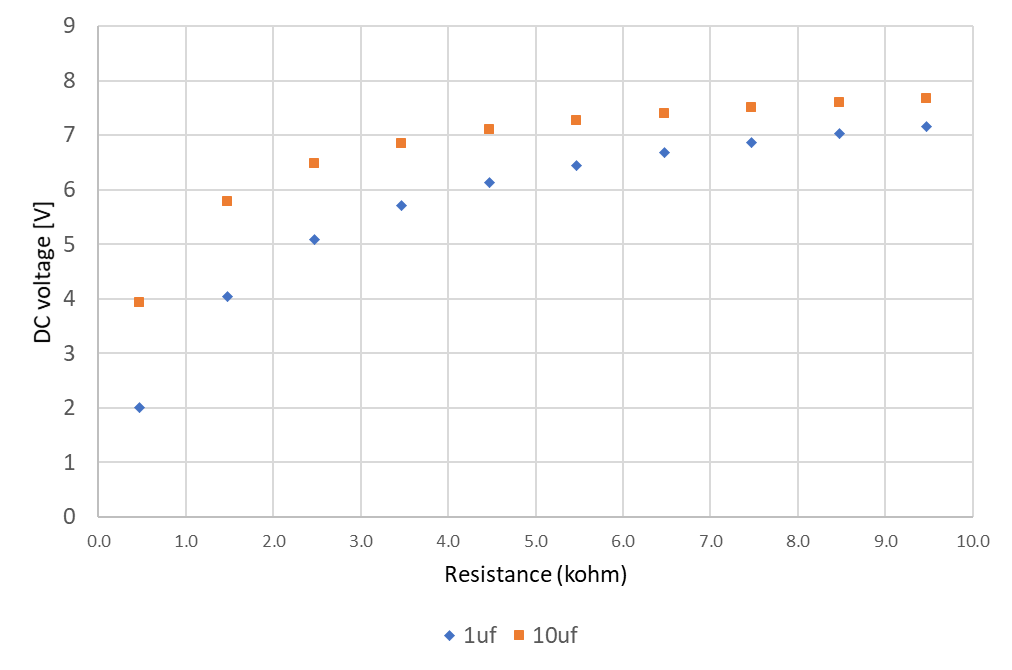
\includegraphics[width=0.7\linewidth]{exp5plotdc}
	\caption{The average DC voltage versus resistance. The higher resistance, the longer charge is retained on the capacitor and the more effective the voltage doubler becomes.}
	\label{fig:exp5plotdc}
\end{figure}

\subsection{Conclusion}
%  conclusion of the exp
The voltage doubler can be used to rectify and double an input ac signal. This relies on diodes operating ideally with minimal drop, and assumes the RC time constant is long enough to allow charge to store within capacitors. It was noted that the larger the capacitor value, the longer a higher voltage would be retained and the more effective the voltage doubler became. Additionally, a higher resistance allowed the voltage to increase. Both of these factors are effects of the RC time constant, which we have used previously.
\end{document}